% !TEX root = ../main.tex
%
\chapter{Results}
\label{sec:result}

This section presents the results of the user study conducted to evaluate the usability of the application.
First the results of the quantitative user experience questionnaire are presented, to gauge the overall user experience.
Following this, the results of the qualitative user testing are analyzed, to provide more detailed insights into the usability of the application.
Finally, the results are integrated and discussed.

\section{User Experience Questionnaire}
\label{sec:result:ux}

Even with the relatively small sample size of 10 participants, the results of the User Experience Questionnaire (UEQ) provide a good overview of the overall user experience.
The scores for the different scales of the UEQ are shown in Figure~\ref{fig:ueq-1}. 

\begin{figure}[htb]
	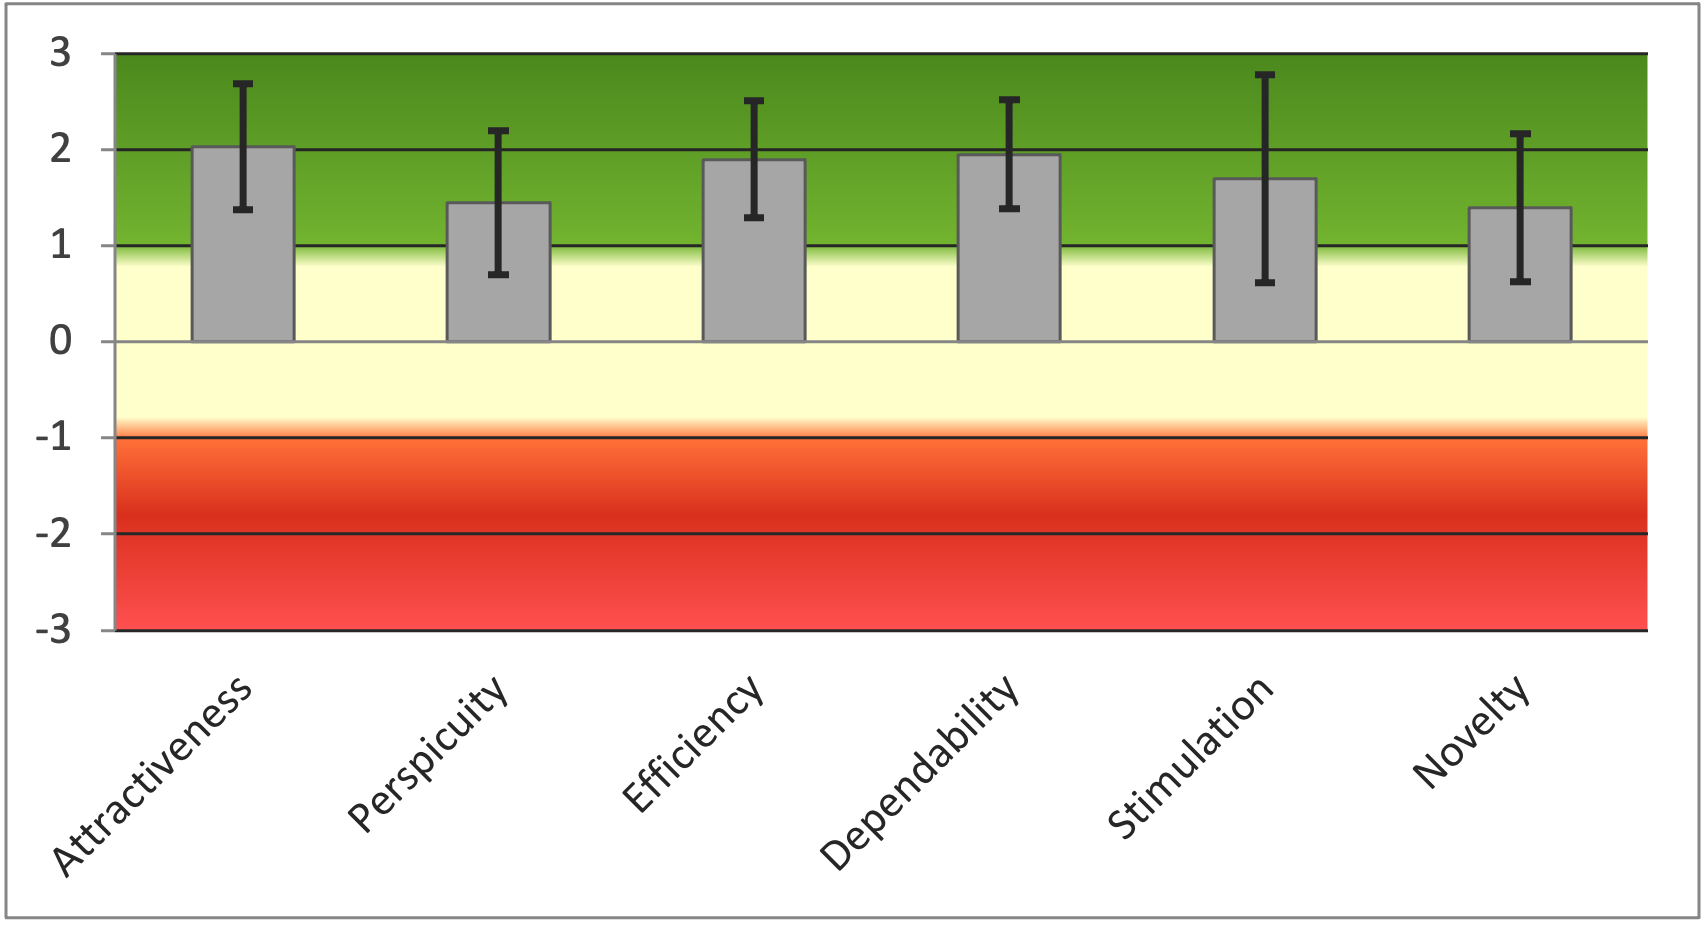
\includegraphics[width=\textwidth]{figures/ueq-1.png}
	\caption{Results of the User Experience Questionnaire}
  \label{fig:ueq-1}
\end{figure}

The \emph{Novelty} scale scores the lowest with a value just below 1 and the \emph{Attractiveness} scale has the highest score with 1.98.
The other scales score between 1.5 and 1.8, indicating a generally positive user experience.

To put the results into perspective, the scores of the UEQ can be benchmarked against the results of other studies.
The UEQ provides a benchmark containing the results of 452 other studies. 
The benchmarking results of the UEQ are shown in Figure~\ref{fig:ueq-2}.
\emph{Attractiveness} and \emph{Dependability} classify as \emph{Excellent}, placing them in the top 10\% of all studies.
\emph{Stimulation} and \emph{Efficiency} both are classified as \emph{Good}, while \emph{Novelty} and \emph{Perspicuity} only classify as \emph{Above Average}.

\begin{figure}[htb]
	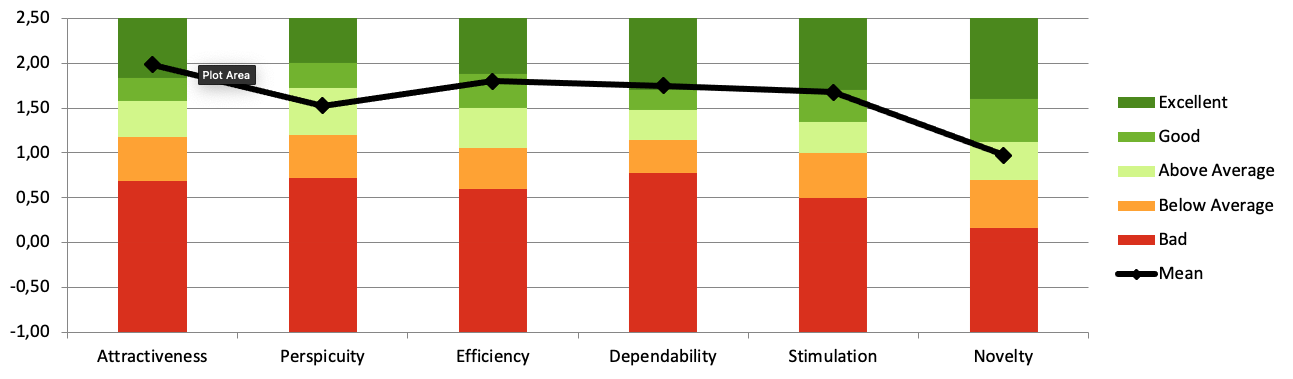
\includegraphics[width=\textwidth]{figures/ueq-2.png}
  \caption{Benchmarking Results of the User Experience Questionnaire}
  \label{fig:ueq-2}
\end{figure}

\todo{specify relation between variance and confidence interval}
The variance of the scores is relatively high, due to the small sample size.
Across the first five scales it is between 0.49 and 0.92, only exceeding 1 for the \emph{Novelty} scale with a value of 1.31.

Table \ref{tab:ueq-summary} provides a summary of the results of the UEQ, besides the mean values and confidence intervals, shown in Figure \ref{fig:ueq-1}, it also includes the standard deviation.
The standard deviation can be interpreted as a measure of agreement between the participants, with lower values indicating higher agreement.
Any value below 0.83 is considered \emph{high agreement}, while values between 0.83 and 1.01 are considered \emph{medium agreement} and values above 1.01 are considered \emph{low agreement}.
Of the six scales, three have a high agreement, two have a medium agreement and one has a low agreement.

\begin{table}[htb]
  \centering
  \begin{tabularx}{\textwidth}{|X|l|l|l|l|l|}
  \hline
      \textbf{Scale} &  \textbf{Mean}  &  \textbf{Conf.} &  \textbf{Conf. Int.} &  \textbf{Std. Dev.} & \textbf{Agreement}\\ \hline
      \textbf{Attractiveness} & 1,983  & 0,445 & 1,538 - 2,428 & 0,718 & high \\ \hline
      \textbf{Perspicuity} & 1,525 & 0,573 & 0,952 - 2,098 & 0,924 & medium\\ \hline
      \textbf{Efficiency} & 1,800 & 0,500 & 1,300 - 2,300 & 0,806 & high \\ \hline
      \textbf{Dependability} & 1,750 & 0,432 & 1,318 - 2,182 & 0,691 & high \\ \hline
      \textbf{Stimulation} & 1,675 & 0,594 & 1,081 - 2,269 & 0,958 & medium \\ \hline
      \textbf{Novelty} & 0,975 & 0,710 & 0,265 - 1,685 & 1,145 & low \\ \hline
  \end{tabularx}
  \vspace{6pt}
  \caption{Summary of the User Experience Questionnaire Results}
  \label{tab:ueq-summary}
\end{table}

\subsection*{Summary}

The analysis of the UEQ results gives some insights regarding the application's user experience. 
Higher scores in the \emph{Attractiveness} and \emph{Efficiency} scales, accompanied by high agreement among participants, indicate that these aspects of the application are both effective and appealing. 
The consistency in these scores suggests that such attributes can be quickly gaged by users, even within the limited timeframe of the user study, leading to a uniformly positive perception.

On the other hand, the lower score and agreement on the \emph{Novelty} scale indicate varied perceptions of the application’s innovativeness. 
This could imply that while the application may not introduce new features or functionalities, it effectively repackages existing ones within an intuitive user interface. 
The moderate novelty score might reflect a use of familiar concepts and interactions, which can reduce the learning curve by leveraging well-understood mechanisms.

However, it is important to note that these findings are based on a relatively small sample size of 10 participants. 
While the results provide valuable insights, they should not be overvalued or considered definitive. 
Caution should be exercised in generalizing these findings without further validation from a larger, more diverse sample.

\section{Findings from Qualitative User Testing}
\label{sec:result:qualitative}

This section presents the findings from the user study conducted to evaluate the user interface of the application. The results are organized into categories reflecting overall impressions, learning curve and accessibility, identified issues, and recommendations for improvement, which now include feature requests.

\subsection*{Overall Impressions}
\label{sec:results:overall_impressions}

Users generally find the interface user-friendly, effective, and aesthetically pleasing, enhancing the user experience across various functionalities. 

\cleanchapterquote{Also es ist auf jeden Fall sehr schönes Tool, also angenehm zum Nutzen.}{Participant 2}{}

\paragraph{User-Friendly} 
Participants highlighted the intuitive layout and ease of navigation within the interface, appreciating how straightforward it was to perform tasks without prior training or extensive help. 
\cite{P1, P2, P4, P5, P7, P8, P10}
% The logical arrangement of elements and minimalistic design were frequently mentioned as factors that reduced cognitive load and facilitated quicker learning and adaptation.
 
\paragraph{Effective} 
The effectiveness of the interface was noted in terms of its responsiveness and reliability. 
Users were satisfied with the speed at which the interface responded to commands and the consistency of its performance during tasks, which helped in building trust and reducing frustration during interactions.
\cite{P2, P4, P7, P8, P10}
 
\paragraph{Aesthetically Pleasing} 
Many users commented on the visual appeal of the interface, mentioning the modern and clean aesthetic that made the experience more engaging. 
\cite{P7, P8, P10}

These aspects collectively contribute to a positive user experience, making the application not only a tool that meets functional needs but also a pleasure to use, thereby encouraging repeated and prolonged engagement.

\subsection*{Learning Curve and Accessibility}
\label{sec:results:learning_curve_accessibility}

% \cleanchapterquote{Also es ist auf jeden Fall sehr schönes Tool, also angenehm zum Nutzen.}{Participant 2}{}

Accessibility and ease of use are the main concerns of the application, driven to reduce the technical knowledge required to enable a broader user base.
This section elaborates on the specific feedback received regarding the short comings and successes of the application in this regard.

\paragraph{Ease of Use}
As mentioned above, the overall user-friendliness was well received by participants across the board.
Feedback from users indicates that the layout and workflow of the application facilitate quick learning and ease of use.
\cite{P4, P5, P7, P8, P10}
The progress indicator as shown in Figure~\ref{fig:design:training-section} was particularly appreciated, as it helped users understand the current state of the application and what steps were required to complete a task.
\cite{P5, P7, P8, P9}

\paragraph{Overwhelming Aspects}
Despite the general ease of use, some users expressed concerns about overwhelming aspects of the interface.
The parameter settings often require a deep understanding of NeRF technology to understand there effects, but this did not hinder the overall usability of the application.
\cite{P5, P7}
The viewer component, while powerful, presents a steep learning curve due to its complexity and the dense presentation of information and controls. 
New users, unfamiliar with NeRF and in particular Nerfstudio, might find this part of the application challenging to navigate initially.
\cite{P2}

\paragraph{Technical Complexity}
Reducing the technical complexity inherent from NeRF applications is crucial in making the application more accessible to a broader audience.
Based on the feedback received from users, that were previously unfamiliar with NeRF, the application requires users to have some level of prior knowledge.
The guided experience and reduced amount of options to configure, was appreciated by certain participant.
It enabled them to quickly get started with the application without feeling overwhelmed.
Most users felt confident, that after a short learning phase, they would be able to use the application effectively.
\cite{P2, P3, P4, P5, P6, P7, P8}
However the feedback indicates a need for an onboarding process or tutorials to help new users overcome initial hurdles and gain confidence in using advanced features.
In contrast, advanced users appreciated the depth of control and customization available.
\cite{P9, P10}
The ability to fine-tune settings through the advanced options was seen as a valuable feature, allowing them to optimize the processes for their specific needs.

\paragraph{Project Management}
Novice users appreciated the similarities to existing project management of a already familiar tool from the film industry. 
\cite{P5}
For experienced users, the abstraction of tedious project management tasks, like file uploads and data organization, was well received.
\cite{P1}
This allowed them to focus on the core tasks of training and rendering, without getting bogged down by administrative overhead.

\paragraph{Technical Language}
One particularly insightful point of concern, was the unfamiliar terminology used, as there exist differences between some terms in the context of NeRF and the film industry. 
\cite{P5}
This can lead to confusion and hinder the learning process, as users struggle to understand the meaning and implications of certain terms.
Adjusting the language used in the application to specifically target the intended audience, can help bridge this gap and further reduce the learning curve.

In summary, the application succeeds in providing new users with access to advanced NeRF tools, while also catering to the needs of experienced users by offering advanced options for customization.

\subsection*{Identified Issues}
\label{sec:results:issues}

% \cleanchapterquote{Also es ist auf jeden Fall sehr schönes Tool, also angenehm zum Nutzen.}{Participant 2}{}

The following issues were identified during the user testing sessions, based on feedback from participants. 
Most of these issues became apparent while participants were performing tasks, and then were further discussed during the post-task interviews.

\paragraph{Unclear Navigation}
Users experienced confusion about navigating through tasks and understanding their progression within the application.
This was particularly evident when having to switch to a different project.
The intended way to navigate to the dashboard was to click on the logo, which was not immediately clear to all users.
Some users succeeded in finding the dashboard after some exploration, while others used browser navigation to return to the dashboard.
\cite{P1, P4, P5, P6, P8, P10}
Some participant also mentioned uncertainties about navigating between the different sections of a project.
The progress indicator can be used to navigate between the different sections, but some users took some time to discover this feature.
\cite{P9}

\paragraph{Inconsistent Wording}
\label{sec:results:issues:inconsistent_wording}
An issue that almost many participants stumbled upon was the inconsistent wording used specifically on the button to start the training process.
In the version of the application used during the user study, the button was labeled \emph{"Start Processing"}, which was confusing to most users.
% This issue highlights the importance of consistent and clear wording throughout the application. 
\cite{P2, P3, P6, P7, P8}

\paragraph{Project Creation}
Similar to the wording issue, the process of creating a new project was not as intuitive as intended.
Many participants encountered a small annoyance when they tried to click on the big plus icon placed in the center of the card, which was not clickable. \fref{fig:design:dashboard}
Although everyone quickly discovered the intended way to create a new project, this issue was mentioned by almost all participants.
\cite{P3, P4, P5, P6, P7, P8}

\paragraph{File Upload}
\label{sec:results:issues:file_upload}
A few participant experienced issues with the file upload process. 
\cite{P1, P4, P6}
The system model is quite complex, as it involves multiple steps and the feedback provided was lacking in some cases.
Before pre-processing can start, the user has to select the input data to use, upload it to the server, wait for the upload to complete before continuing.
Users were not always aware of the progress, and would sometimes continue to the next step before the upload was complete. 

\paragraph{Viewer and Screen Layout}
Feedback indicates a need for a more flexible UI that adjusts to different screen sizes and supports fullscreen modes.
\cite{P10}

\todo{add more details}

\paragraph{Awerness of Progress}
In some cases, users were not aware in what stage of the creation process they were in.
This was somewhat caused by the inconsistent wording (see \ref{sec:results:issues:file_upload}), but also by the high degree of similarity between the pre-processing and training steps.
\cite{P2}

\paragraph{Console Output}
The console output was perceived differently by users. 
Some users appreciated the detailed feedback and insights provided, even with no technical background. \cite{P5}
Others that could not interpret the output, found it useless and distracting. \cite{P3, P4}


\subsection*{Recommendations for Improvement}
\label{sec:results:recommendations}

This section outlines some of the recommendations for improving the application based on the feedback received from participants. 
In contrast to the identified issues, these recommendations are more general and focus on improving the overall user experience.

\paragraph{Enhance Interface Usability}
To address the need for a more personalized and less distracting user interface, the animated background should be able to be disabled.
Additionally, implementing a 'back-to-top' button would streamline navigation, enabling users to quickly return to the top of the page without manual scrolling. 
\cite{P10}

\paragraph{Viewer Customization and Usability Enhancements}
Several enhancements to the viewer are recommended to improve its functionality and usability:

\begin{itemize}
  \item \textbf{Multiple Viewing Modes}: Incorporate the ability to view the cameras perspective, as well as the scene from different angles, providing users with a more comprehensive understanding of the scene. 
  \cite{P5}
  \item \textbf{Advanced Camera Controls}: Introduce adjustable controls for camera speed, motion blur, and the ability to set up speed ramps, to provide users with greater creative control. 
  \cite{P5}
  \item \textbf{Measurement Tools}: Add tools that enable users to take precise measurements within the viewer, useful for detailed scene planning and analysis. 
  \cite{P7}
\end{itemize}

The participants requesting these features were exclusively users with a background in film production, who would include these features in their workflow.

\paragraph{Expand Advanced Settings and Benchmarks}
User with an academic background in NeRF requested the following features, when evaluating the application for their workflow:

\begin{itemize}
  \item \textbf{Support for different NeRF implementations}: Allow users to select different NeRF implementations, providing flexibility and customization options based on their requirements. 
  \cite{P1}
  \item \textbf{Advanced-Advanced Settings}: Provide deeper customization options for experienced users who require fine control over parameters, possibly allowing them to inject custom settings or scripts.
  \cite{P9}
  \item \textbf{Integration of Benchmarking Tools}: Integrate tools like TensorBoard or WandDB to allow users to perform benchmarks, providing insights into model performance.
  \cite{P10}
\end{itemize}


\paragraph{Camera and Shot Management}
Develop a more structured approach to camera and shot management within the application to support complex productions.
Allow users to label and organize different camera shots and paths, making it easier to manage multiple views or scenes within a single project.
\cite{P5}

\paragraph{Tighter Integration of Viewer}
One participant suggested a tighter integration of the viewer with the rest of the application.
Building the viewer controls directly into the interface, instead of inserting the viewer as a separate component, to provide a more seamless experience.
\cite{P9}

\subsection*{General Feedback}

\paragraph{Lack of Modification Options}
Creatives would like to see more options for modifying the scene, such as adding objects or changing the lighting.
\cite{P3}

\todo{add more details}

\paragraph{Use Cases}
Some participants saw no potential use cases for the application or NeRF in general in their current workflow. 
\cite{P3}
Others cited the limitation to static scenes as a major drawback, as they require dynamic scenes for their projects. 
\cite{P4, P5}
But the possibility for stylized and 'impossible' camera movements was inspiring application in advertisement and music videos. 
\cite{P4}
Pre-visualization was also mentioned as a potential use case, as it allows for quick and easy scene creation that can be used for planning and storyboarding. 
\cite{P4}


\section{Integration and Findings}
\label{sec:result:findings}
\todo{Add integration and findings}

